% \documentclass{ijsra}
\def\IJSRAidentifier{\currfilebase} %<---- don’t change this!
\def\submission{}%YYYY-MM-DD
\def\acceptance{}%YYYY-MM-DD
%-------Title | Email | Keywords | Abstract-------------
\def\shorttitle{ICAHM 2017 Meeting Review}
\def\maintitle{ICOMOS International Committee on Archaeological Heritage Management (ICAHM) 2017 Annual Meeting: A Review}
\def\cmail{}
\def\keywords{Conference review, student participation, International Committee on\\ Archaeological Heritage Management}
%\def\keywordname{}%<--- redefine the name “Keywords“ in needed language
\def\abstract{The ICOMOS International Committee on Archaeological Heritage Management (ICAHM) Annual Meeting is an event where heritage experts, academic professionals and students meet to share, discuss and advance the management of archaeological heritage and archaeological research all over the world. The ICAHM 2017 Annual Meeting was held in Bagamoyo, Tanzania thereby becoming the first ICAHM meeting to be held in Africa. The theme of the meeting was \emph{Archaeological Heritage in Sub-Saharan Africa, International Trade Routes, and Conservation} which encouraged collaboration in archaeological research and archaeological heritage management in Sub-Saharan Africa. Here, we review this annual meeting alas with a bias towards students’ participation.}
%--------Author’s names------------
\def\authorone{Humphrey Nyambiya, Barpougouni Mardjoua,\\ and Ashley Maganzo}
%-------Biographical information-------------
\def\bioone{}
%------University/Institution--------------
\def\affilone{no affil}

\begin{filecontents}{\IJSRAidentifier.bib}
	}
\end{filecontents}
\IJSRAopening%<---- don’t change this!
%-------
\lettrine{T}{h}e International Committee on Archaeological Heritage Management (hereafter referred to as ICAHM) is a scientific committee of the non-governmental International Council of Monuments and Sites (ICOMOS). ICOMOS is responsible for the evaluation of all nominations of cultural properties against the criteria laid down by the World Heritage Committee. ICAHM advises ICOMOS and the World Heritage Committee on matters that pertain to all aspects of the management of archaeological sites and landscapes (\url{http://icahm.icomos.org}). This objective is fulfilled through promotion of the understanding of the importance of the archaeological heritage to the general public, government institutions and all stakeholders. Thus ICAHM promotes the development, and propagation of best practices for both archaeological research and cultural resource management.

ICAHM is interested in all archaeological sites, landscapes and related resources in the world as such, it collaborates with international, national, regional and local organizations that pursue similar goals. One of the roles of ICAHM is to review nomination dossiers for cultural sites nominated for World Heritage listing. Another key role for ICAHM is to develop a network of professionals who share varied experience essential to the management of archaeological heritage and research. ICAHM seeks to achieve these goals through Annual Meetings and workshops to discuss best practices for a) management of archaeological heritage sites, b) archaeological research, c) aspects of cultural resource management. In the past, the Committee has arranged Annual Meetings in 2012 in Cuzco, Peru; 2014 in Jishou, China; 2016 in Salalah, Oman and most recently 2017 in Bagamoyo, Tanzania, which is the focus of this review.

The 2017 ICAHM Annual Meeting was held in the historic town of Bagamoyo, Tanzania. This conference was first in the history of ICAHM to be in Africa. The theme for the conference was \emph{Archaeological Heritage in Sub-Saharan Africa, International Trade Routes, and Conservation}, which stimulated sessions, oral presentations and poster presentations that were important to the international community. From this theme, emphasis was on the conservation and sustainability of archaeological heritage in Sub-Saharan Africa particularly towards Sustainable Development Goals (SDGs). Ultimately, this conference theme attracted 90 delegates from about 30 countries.

\IJSRAsection{Conference Sessions}

ICAHM hosted this Annual Meeting in Tanzania to discuss Sub-Saharan Africa and International Trade Routes. Eastern Africa, Tanzania in particular has rich paleoanthropological sites. These include Olduvai Gorge and the Laetoli World Heritage Sites in the Ngorongoro Conservation Area carry the remains of \emph{Australopithecus boisei}, \emph{Australopithecus aethiopicus} and \emph{Australopithecus afarensis}. In addition, \num{3.6} million years old hominin footprints have been discovered in the country. Tanzania is known for coastal sites such as Kilwa Kisiwani and Zanzibar. These are attached with rich tangible and intangible heritage aspects. The island has been depicted historically and archaeologically as having connections within Africa, the Middle East and the Far East, \emph{i.e.}, Southeast Asia.

The conference proceedings started with a keynote address from Dr. Webber Ndoro on the Africa Initiative programme (\cref{fig:ICAHM_Figure_01a}).  The Africa Initiative programme came as a realization that there are few World Heritage Sites from Africa on the World Heritage List given the number of sites that have the potential to become World Heritage sites from the continent. Thus, ICAHM launched the Africa Initiative programme in 2011 with the aim of increasing World Heritage Sites from Africa. The wish of ICAHM to increase the number of sites on the World Heritage List from Africa is shown by the fact that it will be one of the 2018 Annual Meeting session themes to be held in Sicily, Italy. Thus, there is need for concerted efforts among archaeologists, cultural heritage practitioners and related professionals for the Africa Initiative programme to materialize.

%FIGURE 1a: Webber Ndoro, Africa Initiative
\begin{figure}[!htb]
	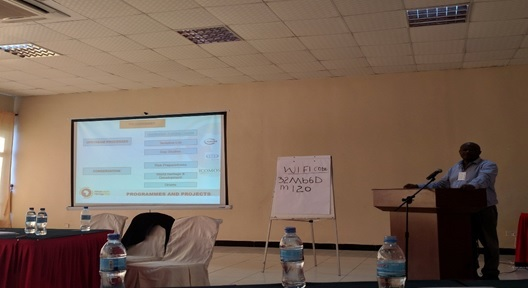
\includegraphics[width=\linewidth]{ICAHM_Figure_01a}
	\caption{Dr. Webber Ndoro discussing the Africa Initiative programme during the keynote address.
		{\normalfont\scriptsize \\ \copyright\
			Humphrey Nyambiya, Barpougouni Mardjoua, and Ashley Maganzo %\shortauthor
	}}
	\label{fig:ICAHM_Figure_01a}
\end{figure}

The conference themes were as follows:
\begin{enumerate}
	\item Trade Routes: Africa’s role as a gateway to the rest of the World
	\item Conservation and sustainable use of paleoanthropological sites
	\item World Heritage Sites as Sources for Sustainable Development
	\item Maritime Underwater Cultural Heritage
	\item Digital Technologies and Archaeological Heritage Management
\end{enumerate}

Research papers of various topics were presented under the themes of the conference by different presenters from all over the world. In the Maritime Underwater Cultural Heritage session, exchange of expertise among professionals was encouraged as there is lack of training and resources especially in Africa.

\IJSRAsection{Student Participation at the ICAHM 2017 Conference}

Analysis of the ICAHM conference database has shown that its Annual Meeting is one place where experts in archaeological heritage management around the world meet, discuss and map ways forward to achieves the goals and mission of ICAHM. The conference theme and the 2017 Annual Meeting was well received with 90 participants from different parts of the world, with about 30 countries being represented. Of the 90 people who attended the conference, only 9 of them were students from different institutions and countries (\cref{tab:ICAHM_Table_01}, \cref{fig:ICAHM_Figure_01b}).

Registration fees were a requirement and were demarcated between foreign participants from developed countries, foreign participants from developing countries, participants from Tanzania, Students from developed countries, Students from developing countries and students from Tanzania. The registration fee included all the conference proceedings as well as a GIS workshop for interested participants. Registration fees for students were US \$75 for students from developed countries, \$40 for students form developing countries and \$20 for students from Tanzania, to participate in the conference proceedings. Thus, this shows that the registration fee for students to participate in ICAHM’s Annual Meetings is affordable to many students.

\begin{table}[]
	\centering
	\caption{Statistics on students attending ICAHM conferences}
	\label{tab:ICAHM_Table_01}
	\begin{tabular}{llll}
		Conference meeting & Year & Number of students & Total participants \\
		Cuzco-Peru         & 2012 & 22                 & 170                \\
		Jishou-China       & 2014 & 12                 & 105                \\
		Salalah- Oman      & 2016 & 1                  & 80                 \\
		Bagamoyo-Tanzania  & 2017 & 9                  & 90
	\end{tabular}
\end{table}

%FIGURE 1b: ICAHM attendances
\begin{figure}[!htb]
	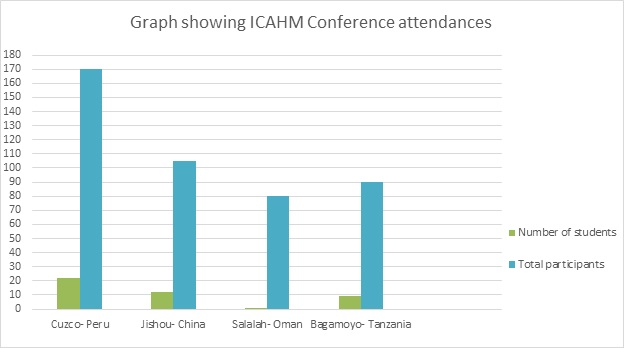
\includegraphics[width=\linewidth]{ICAHM_Figure_01b}
	\caption{Graphical presentation of the ICAHM conference attendances.
		{\normalfont\scriptsize \\ \copyright\
			Humphrey Nyambiya, Barpougouni Mardjoua, and Ashley Maganzo %\shortauthor
	}}
	\label{fig:ICAHM_Figure_01b}
\end{figure}

Students were given an opportunity to participate and presented papers in the following session themes: Trade Routes: Africa's Role as a Gateway to the Rest of the World; World Heritage Sites as Sources for Sustainable Development; Digital Technologies; and Archaeological Heritage Management. However, a major challenge faced by students, was particularly on raising funds to attend the conference. Some students who had their papers accepted after the call for papers failed to attend and present their papers as they had no funds to travel to Bagamoyo, Tanzania. But nonetheless, those who attended benefitted immensely from the event and learnt a lot about archaeological site management from the various sessions held.

Although the number of students increased as compared to student attendances in Oman, the attendance of students to ICAHM conferences is still low. Moreover, there is need for archaeological and heritage professionals and experts to integrate students in the planning of such events and also to encourage them to attend conference meetings of this kind because most of the experts and professionals work in institutions with students in either way. It is a thing of the past for professionals and experts to work in isolation with students. A piecemeal integration between these two would go a long way in addressing a major concern among students.

\IJSRAsection{Workshop: GIS and Direct Detection of Archaeological Sites in a Landscape Context Using Aerial and Satellite Imagery and Open Source Software}

This workshop was held as part of ICAHM 2017 Annual Meeting with the aim of locating archaeological sites using GIS. The workshop was facilitated by Dr.~Douglas C. Comer where the use of GIS in archaeology was accentuated. In this workshop, GIS Software was used. For purposes of demonstration and for time constraints, four natural World Heritage Sites in Tanzania were located. The four are Kilimanjaro National Park, Ngorongoro Conservation Area, Selous Game Reserve and Serengeti National Park. To identify these sites, aerial photographs were used in association with the coordinates of the sites.

In archaeological prospection, GIS is used to locate sites where vegetation might be a pointer to an archaeological site. In most instances, vegetation with stunted growth may be a result of past habitation where the resources used in habitation impede growth of vegetation. Depending on the nature of the vegetation, greener vegetation might also indicate an archaeological site or past areas of activity. For example, a place which was once used as an animal kraal might have greener vegetation than its surrounding area. However, GIS in archaeology has been criticized for being environmentally deterministic, thereby dehumanizing the past. But in any way, there is a close relationship between the environment and people regardless of which factor affects the other. Similarly, in a world where technology seems to dominate all aspects of human existence, there is need to fully embrace this technique.

\IJSRAsection{Guided walk through Bagamoyo}

After the workshop on GIS and Direct Detection of Archaeological Sites in a Landscape Context Using Aerial and Satellite Imagery and Open Source Software, the conference delegates had the opportunity of a guided walk by a representative of the Tanzanian Antiquities Department through the historic town of Bagamoyo. The places visited included the Germany Boma, the fish market and the curio shop (Bagamoyo Art Market). The Germany Boma was built by the German in 1897 as the colony’s central administrative office and residence of the colonial administrator (\cref{fig:ICAHM_Figure_02}). It is associated with the slave trade. The fish market in Bagamoyo is on the shores of the Indian Ocean. The inhabitants of Bagamoyo are earning a living from this fish market. The curio shop visited by the conference delegates’ shows works of art. Some of the products sold are carvings, pieces of adornments, picture paintings and drawings (\cref{fig:ICAHM_Figure_03}). In any case, the products have a traditional aspect added to them.

%FIGURE 2: Germany Boma
\begin{figure}[!htb]
	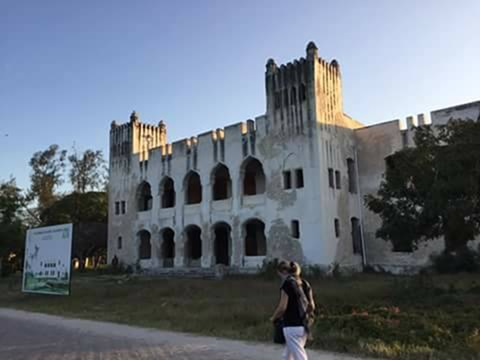
\includegraphics[width=\linewidth]{ICAHM_Figure_02}
	\caption{The Germany Boma.
		{\normalfont\scriptsize \\ \copyright\
			Humphrey Nyambiya, Barpougouni Mardjoua, and Ashley Maganzo %\shortauthor
	}}
	\label{fig:ICAHM_Figure_02}
\end{figure}

%FIGURE 3: Bagamoyo
\begin{figure}[!htb]
	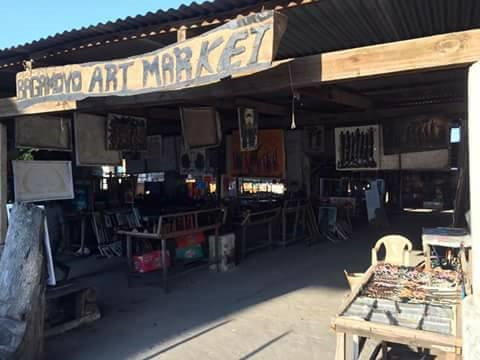
\includegraphics[width=\linewidth]{ICAHM_Figure_03}
	\caption{Curio shop (Bagamoyo Art Market).
		{\normalfont\scriptsize \\ \copyright\
			Humphrey Nyambiya, Barpougouni Mardjoua, and Ashley Maganzo %\shortauthor
	}}
	\label{fig:ICAHM_Figure_03}
\end{figure}

As a result of this tour, there was a general satisfaction among conference delegates of the historicity of this town. Indirectly, this tour reiterated the sentiment made by Dr.~Ndoro in his keynote speech that there is need for concerted efforts among heritage professionals to nominate Bagamoyo on the World Heritage List.

The ICAHM Meeting was preceded and succeeded by excursions. Here we would like to outline the main phases of the post-conference excursion. The conference ended on October 5 with a group excursion to the Village Museum and National Museum in Dar es Salaam. In the National Museum we were offered the unique opportunity to visit the vault where Prof.~Charles Musiba showed the participants various hominid discoveries by the famous palaeoanthropologists Louis and Mary Leaky.  From 6 to 9 October 2017, a post-conference excursion took place where 30 participants had a tour to Karatu where they spent two nights and visited the Laetoli Footprints and Olduvai Gorge in the Ngorongoro Conservation Area. The participants visited the Ngorongoro Crater on 7 October. The post-conference excursion was as great as the conference, and the participants appreciated it.

\IJSRAsection{Recommendations}

Since one of the functions of ICAHM is to develop and enhance a network of professional archaeologists and archaeological site managers for the purpose of transmitting theoretical and practical skills and encouraging high standards and best practices for a) management of archaeological sites and resources; b) archaeological research; and c) aspects of cultural resource management, we recommend that students be more involved in ICAHM programs. This can be through the creation of student membership or an ICAHM student forum as they are upcoming experts in the field. This is because, currently, membership to ICAHM is confined to experts and professionals. Regarding a student forum, ICAHM’s Annual Meetings could involve students in the planning of the same such that during a conference there is time specifically dedicated to students. This can be time for students, professionals, and experts to meet and discuss the prospects of their careers. We believe there is more that students can contribute towards the cause of ICAHM through programs aimed at promoting the preservation, conservation and utilization of archaeological resources as well as research.

To most students particularly from developing countries, international travel is expensive such that most students cannot afford it. Since ICAHM does not charge a membership fee, there are usually no funds available for travel grants for conference attendees.  Ideally, this should be a different situation all together when it comes to students. We recommend that ICAHM makes provisions for travel grants especially to students. The absence of travel grants could be one of the major setbacks resulting in decreased number of student participation in ICAHM’s conferences. Overall, we believe that such a lacuna can be filled if the above recommendations can be adopted.

\IJSRAsection{Conclusion}

The ICAHM Annual Meeting held October 2 to 5, 2017 was an excellent meeting and exchange opportunity for participants. The whole of activities carried out ensures that we keep a good memory of the colloquium and that the conference was an excellent crucible of initiation and training on the management of cultural heritage. In the future, we hope there will be an increase in student participation at ICAHM Annual Meetings.

\IJSRAsection{Acknowledgments}

Mardjoua would like to humbly thank the African World Heritage Fund for the travel grant to participate in the conference, FPMA, and Mr. Souayibou Varissou. Nyambiya would like to thank The Mirror International Research Institute (TMIRI) for funding his stay in Tanzania. We would like to thank Annemarie Willems and Simon Makuvaza for comments to the earlier draft. Finally, we would like to thank the organizers of the conference and Friends of ICAHM.

\IJSRAclosing%<---- don’t change this!
